% ============================================================
\section{Proactive Tutoring}
\label{sec:proactive}
% ============================================================

\begin{figure*}[t]
    \centering
    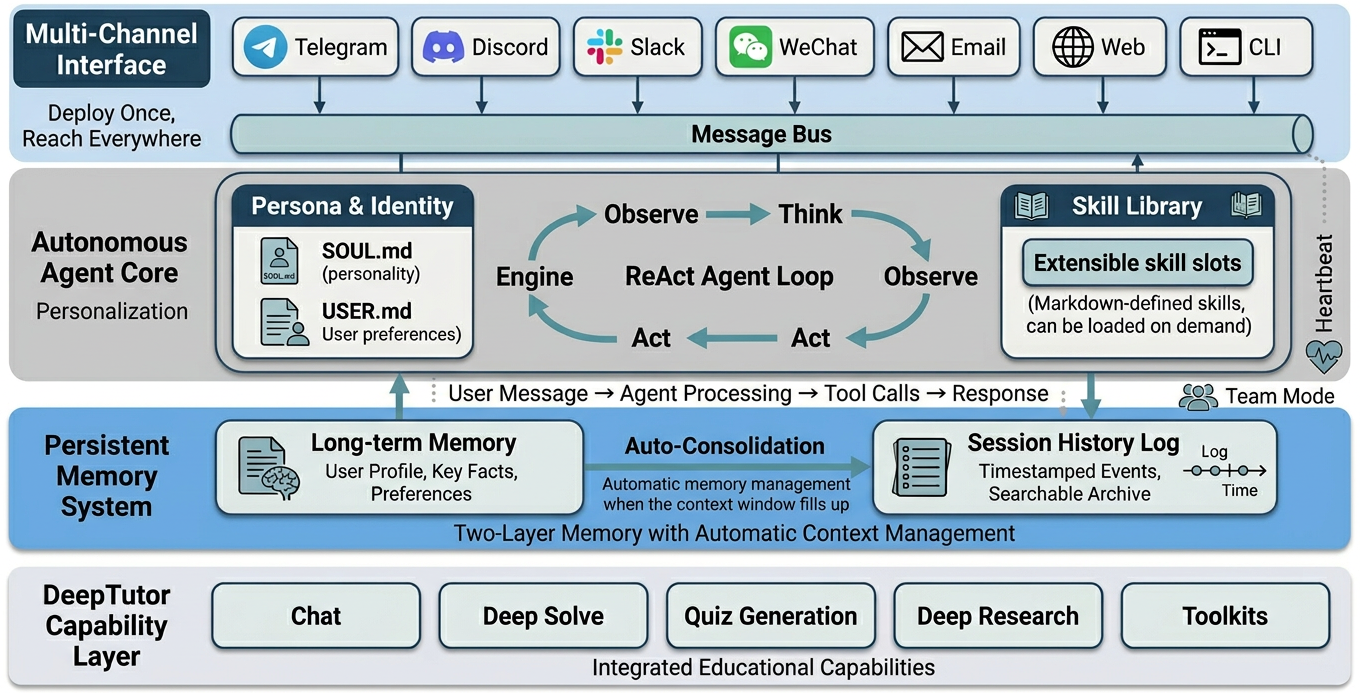
\includegraphics[width=\textwidth]{figures/tutorbot.png}
    \caption{TutorBot architecture. Four layers from top to bottom: a \emph{multi-channel interface} connecting twelve messaging platforms through a unified bus; an \emph{autonomous agent core} with a customizable persona (Soul) and extensible skills; a \emph{persistent memory system} with automatic consolidation; and the \emph{shared DeepTutor runtime} exposing the full tutoring stack as reusable services.}
    \label{fig:tutorbot}
\end{figure*}

The personalized tutoring capabilities described in~\S\ref{sec:responsive}, however comprehensive, remain largely learner-initiated.
They are typically accessed through a web interface or CLI, which means the learner must decide when to engage and which entry point to use.

This creates two practical limitations.
First, \emph{interaction friction}: the learner must remember to return, open the right interface, and formulate the next request.
Second, \emph{context fragmentation}: a student who uses the web interface on a laptop, the CLI from a terminal, and a messaging app on a phone can easily end up with disconnected sessions that do not share state.

TutorBot is our design for this proactive layer.
Rather than introducing a second tutoring system, it reuses the tutoring workflows described in~\S\ref{sec:responsive} in a longer-horizon, multi-channel setting.
This section describes four design decisions, illustrated in Figure~\ref{fig:tutorbot}: enabling each bot to autonomously invoke the existing tutoring workflows through a persistent agent loop~(\S\ref{sec:agentloop}), extending behavior through skills~(\S\ref{sec:skills}), supporting multiple specialized bots in parallel~(\S\ref{sec:multibot}), and unifying context across channels~(\S\ref{sec:channels}).

% ------------------------------------------------------------
\subsection{From Capability Execution to Autonomous Agency}
\label{sec:agentloop}
% ------------------------------------------------------------

The first requirement is that every workflow available in the tutoring dimension, including problem solving, question generation, collaborative writing, deep research, and guided learning, must be invocable by an autonomous bot, not only by a human clicking a button.

TutorBot achieves this through runtime reuse: it invokes the same tutoring workflows that power the web interface, through the same orchestrator and personalization backbone.
An adapter layer translates between the bot's conversational message format and \textsc{DeepTutor}'s unified context structure.
Each TutorBot instance runs in-process within the \textsc{DeepTutor} server, sharing the same LLM configuration, knowledge-base indices, and provider connections, with no separate deployment required.
The CLI exposes bot management as a first-class entry point, and bot-initiated conversations flow through the same pipeline as web or messaging interactions.

At the core of each instance is an autonomous agent loop (Algorithm~\ref{alg:tutorbot} in Appendix~\ref{app:tutorbot}) following the observe--think--act paradigm (cf.\ Figure~\ref{fig:tutorbot}, center).
Each inbound message triggers three phases: \emph{context assembly} weaves conversation history, persona definition, skill descriptions, and long-term memory into the agent's working state; \emph{reasoning} invokes tools iteratively until the problem is resolved or a budget is exhausted; and \emph{dispatch} sends the response back through the originating channel.

Two design choices distinguish this loop from a standard ReAct agent.
First, \textbf{persistent two-layer memory} (cf.\ Figure~\ref{fig:tutorbot}, bottom-left): TutorBot maintains a long-term user profile alongside a searchable session history log.
An automatic consolidation mechanism monitors context-window pressure and distills the oldest messages into both layers before the window overflows, enabling coherent interactions across arbitrarily long trajectories.
Second, \textbf{high-level tutoring actions} (cf.\ Figure~\ref{fig:tutorbot}, bottom): beyond low-level primitives, TutorBot can invoke complete tutoring services such as RAG-grounded explanation, deep reasoning, sandboxed code execution, and academic paper search as first-class actions within its reasoning loop.

% ------------------------------------------------------------
\subsection{Unbounded Extensibility via Skills}
\label{sec:skills}
% ------------------------------------------------------------

The tutoring capabilities cover a broad range of learning tasks, but a proactive agent must also support workflow-specific behaviors that are not appropriate to hard-code into the core loop, such as study scheduling, repository monitoring, or recurring report generation.

TutorBot achieves this extensibility through \emph{skills}, self-contained declarative modules that extend the bot's repertoire without modifying core code (cf.\ Figure~\ref{fig:tutorbot}, right).
Each skill is a natural-language specification comprising four elements: \emph{triggers} that tell the agent when to activate the skill, step-by-step \emph{instructions} guiding the agent's behavior, a declaration of the \emph{tools} required, and optional executable \emph{scripts} for complex operations.
Skills function as curriculum for the agent: they teach the LLM how to combine its existing tools in new ways, much as a human tutor might learn a new teaching technique by reading a pedagogical guide.

Built-in skills bridge TutorBot to the full tutoring stack, including problem solving, question generation, deep research, knowledge-base management, and learner memory, while utility skills extend it with scheduling, summarization, and document management.
Skills are loaded from two sources, with workspace-level overrides taking precedence over built-in defaults to enable per-bot customization.

A \emph{skill-creator} meta-skill further allows the bot to author new skills at runtime: when a recurring workflow is not covered by the existing library, the bot can propose, create, and install a new skill.
This mechanism keeps the proactive layer open-ended without requiring frequent modifications to the underlying infrastructure.

% ------------------------------------------------------------
\subsection{Collective Intelligence via Multi-Bot Parallelism}
\label{sec:multibot}
% ------------------------------------------------------------

Complex learning scenarios, from exam preparation to multi-faceted research, benefit from parallel specialized agents.
A single \textsc{DeepTutor} deployment can host multiple independent TutorBot instances, each with its own persona, skill configuration, proactive schedule, and conversation history, while all bots share the same knowledge bases and tutoring runtime.

\paragraph{Personality and Specialization via Soul Templates.}
Each bot's identity, including communication style, expertise scope, and behavioral constraints, is defined through structured \emph{Soul templates} (cf.\ Figure~\ref{fig:tutorbot}, left).
A registry of pre-built templates enables rapid instantiation of specialized agents such as a patient math tutor, a research assistant, a language practice partner, or an exam preparation coach.
Specialization goes beyond surface-level persona: a math tutor bot foregrounds problem-solving and question-generation skills, while a research assistant bot prioritizes literature synthesis and summarization.
The learner thus interacts with a team of specialized agents, each optimized for a particular cognitive task.

\paragraph{Proactive Autonomy.}
Each bot runs a heartbeat service that periodically wakes the agent to evaluate whether proactive action is warranted, for instance checking whether the student has completed a scheduled review, whether a daily practice problem should be generated based on active weaknesses, or whether new papers added to the knowledge base merit summarization.
The LLM itself decides whether to act or defer, reducing unnecessary activations while allowing the system to initiate follow-up when the learner may benefit from it.
A scheduling service supports one-time, recurring, and cron-expression-based tasks that the bot can create dynamically, enabling it to adapt its proactive cadence to the learner's rhythm.

\paragraph{Self-Evolution.}
Because each bot operates in a mutable workspace, it can modify its own configuration over time.
The memory consolidator continuously refines the bot's understanding of the student, the skill-creator produces new behaviors in response to emergent needs, and the proactive schedule adapts to engagement patterns.
Each bot therefore evolves independently, acquiring new skills, refining its persona, and adjusting its proactive cadence, all without affecting other bots in the same deployment.

% ------------------------------------------------------------
\subsection{Unified Context across Channels and Devices}
\label{sec:channels}
% ------------------------------------------------------------

TutorBot embodies a ``deploy once, reach everywhere'' principle: a single bot instance connects to twelve channel adapters spanning consumer messaging (Telegram, Discord, WhatsApp, QQ), enterprise platforms (Slack, Feishu, DingTalk, WeCom), open protocols (Matrix, Email), and self-hosted solutions (MoChat), all behind a unified message bus.

More importantly, all channels share the same backend context.
A student who uses the web interface in the morning, the CLI in the afternoon, and Telegram in the evening interacts with one continuous thread: the same trace forest, learner profile, and personalization context span all entry points.

\paragraph{Discussion.}
The four design dimensions of the proactive layer, namely autonomous capability composition, skill-based extensibility, multi-bot parallelism, and unified cross-channel context, define how the same personalized tutoring capabilities can be deployed in longer-horizon settings.
Our claim is not that this layer is fully evaluated in the present report, but that it provides a concrete systems design for extending a validated tutoring core into proactive, context-unified agents.
We view this as one of the primary insights that a technical report format allows us to share: a detailed architectural blueprint that can inform future implementations and evaluations.
